\chapter{Trabalhos Correlatos}

Para prover serviços inteligentes para \textit{SmartSpaces} é necessário adquirir informações de contexto, informações sobre a pessoas no ambiente e suas interações. Informações como número de pessoas, identidade, localização, postura, orientação da cabeça, entre outros.

Neste capítulo analisaremos alguns projetos que procuram obter informações de contexto como esta. De modo mais específico, informações sobre a identidade e localização das pessoas em um \textit{SmartSpace}.

\section{Projeto CHIL}

O Projeto CHIL (\textit{Computers in the Human Interaction Loop}) é composto por um time de quinze laboratórios internacionais de pesquisa acadêmica e industrial . Eles colaboram entre si no desenvolvimento de serviços que visam ajudar as pessoas de forma proativa durante suas atividades diárias e, em particular, durante sua interação com as outras pessoas. 

Alguns dos protótipos que foram desenvolvidos no projeto incluem um \textit{workspace} perceptivo e colaborativo, diversos serviços que facilitam a colaboração em reuniões e em salas de palestras, e um sistema perceptivo de assitência a um escrtitório virtual~\cite{chil}.

\subsection{Rastreamento e Lozalização de Pessoas}

A pesquisa sobre rastreamento de pessoas foi focada principalmente no rastreamento de pessoas dentro de \textit{SmartSpaces}. O objetivo desse monitoramento foi determinar, para todos os pontos no tempo, as coordenadas dos ocupantes do \textit{SmartSpaces} na cena em relação a uma \textit{frame} de coordenadas. O que contradiz com a maioria das pesquisas de rastreamento visual, onde somente as coordenadas na imagem  são estimadas~\cite{chil}.

Os sensores usados no \textit{SmartSpace} incluem~\cite{chil}:
	
	\begin{itemize}
		\item um mínimo de quatro câmeras fixas instaladas nos cantos da sala, com campos de visão sobrepostos;
		\item uma câmera com grande ângulo de visão fixa com vista para o quarto inteiro;
		\item três arrays de micrfones em forma de T de 4 canais;
		\item um microfone de Mark III de 64 canais;
	\end{itemize}

Essa grande quantidade de sensores disponíveis pode ser vista como uma vantagem, pois podem oferecer uma grande redundância nas informações capturas que podem ser exploradas pelos algoritmos usados. Porém, isso pode também ser visto como um grande desafio, pois surgem problemas como sincronização dos dados, transferência de processamento distribuído, fusão de espaço-temporal, entre outros.

Do ponto de vista do áudio, é importante mencionar que o Projeto CHIL representa uma das primeiras tentativas de realizar e avaliar sistematicamente rastreamento acústico com uma rede distribuída de microfones~\cite{chil}.
	 
O sistema de rastreamento e localização foi amplamente testado usando os dados dos seminários e reuniões CHIL~\cite{chil}.

Durante o projeto, muito progresso foi feito partindo de sistemas de única modalidade com a inicialização manual ou implícita, usando recursos simples, o que implica várias etapas de processamento manualmente concatenadas offline e acompanhamento de no máximo uma pessoa, para um sistema totalmente automático, com auto-inicialização, em tempo real, usando uma combinação de recursos, fusão dos \textit{streams} de vários sensores de áuido e video e capaz de rastrear alvos múltiplos~\cite{chil}.

Sobre os algoritmos de rastreamento visual, duas abordagens principais foram seguidas pelos vários sistemas de rastreamento desenvolvidos~\cite{chil}:
	
	\begin{enumerate}
		\item uma abordagem baseada em modelos, em que um modelo 3D do objeto rastreado é mantido.
		\item  uma abordagem orientada a dados, onde sistemas de rastreamento 2D operam de forma independente sobre os diferentes ângulos de visão das câmeras e os dados do rastreamento pertencentes a um mesmo alvo são coletados no formato de um rastreamento 3D.
	\end{enumerate}

 Em termos de desempenho, a abordagem baseada em modelos geralmente prevê uma melhor acurácia, mas menos precisão do que a abordagem orientada a dados. O tratamento das oclusões e da associação dos dados dos sistemas de rastreamentos independentes são as desvantagens do modelo orientado a dados. Para diminuir o impacto desses problemas, começaram a detectar e rastrear rostos em vez de corpos inteiros~\cite{chil}.

% Sobre os algoritmos de rastreamento por áudio, três abordagens principais foram seguidas~\cite{chil}:
	
	% \begin{enumerate}
	% 	\item abordagens que dependem do cálculo de um campo de coerência global mais ou menos grosseiro, em que o rastreamento dos picos de correlação é realizada;
	% 	\item abordagens filtro de partículas, que estima a posição da pessoa que fala através de um conjunto de amostras e medições dos sinais acústicos observados dado a cada amostra hipóteses sobre a posição;
	% 	\item abordagens que se alimentam dos atrasos de chegada calculados entre os pares microfone como observações para um rastreador probabilístico.
	% \end{enumerate}

Sobre os algoritmos de rastreamento por áudio, três abordagens principais foram seguidas. Entre elas, a que teve a melhor performance foi um sistema baseado em um \textit{Joint Probabilistic Data Association Filter}, que mantém o controle de uma série de fontes de áudio, incluindo fontes de ruídos, resolvendo associações dos dados e atualizando o conjunto de posições~\cite{chil}.

As abordagens de rastreamento por meio de áudio e vídeo foram combinas em um rastreamento multimodal. Esse rastreamento multimodal é, notavelmente, baseado em filtro de partículas uma vez que permitem uma integração flexível de recursos através dos sensores~\cite{chil}.

No rastreamento multimodal, era esperado que a fusão dos diferentes tipos de dados proveria resultados mais precisos, eliminando, assim, os efeitos de decisões erradas tomadas por algum rastreamento monomodal. Porém, não aconteu o que se esperava. O rastreamento multimodal é altamente dependente das tarefas e dados em mãos, e exige um cuidadoso equilíbrio na disponibilidade e qualidade dos dados~\cite{chil}.

\subsection{Identificação das Pessoas}


A fim de realizar identificação de forma natural e implicita, os sensores distribuídos no ambiente devem monitorar continuamente o espaço, e captura de dados áudio-visual das pessoas discretamente quando eles aparecem. Ou seja, o sistema de identificação de pessoas
deve operar em segundo plano, sem necessitar de atenção e cooperação das pessoas. Dependendo da localização de uma pessoa e sua distância dos sensores, os dados recebidos podem variar~\cite{chil}. 

Para reconhecimento facial, o sistema utiliza sequencias de imagens fornecidas pelas várias câmeras no \textit{SmartSpace}. A cada $\displaysyle 200ms$ imagens das ``caixas delimitadoras das faces'' e posições dos centros dos olhos são fornecidas, como exemplificado na Figura \ref{chil}. As faces, então, são alinhadas utilizando os centros dos olhos ou utilizando as ``caixas delimitadoras das faces''. Para obter robustez contra alguns erros, o sistema gera algumas imagens alinhadas adicionais modificando rótulos dos centros dos olhos ou os rótulos das ``caixas delimitadoras das faces''~\cite{chil}.

	\begin{figure}[hbt]
		\begin{center}
			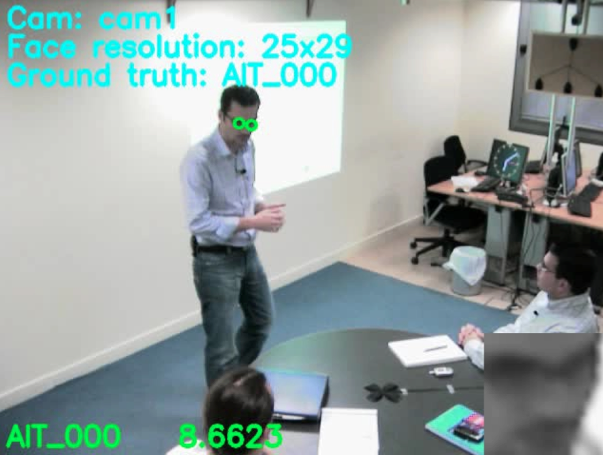
\includegraphics[scale=0.4]{figuras/3.TrabalhosCorrelatos/chil.png}
		\end{center}
		\caption{Exemplo do sistema de indetificação facial do Projeto CHIL. No canto inferior direito, pode-se observar a imagem da face extraída~\cite{chil}.}
		\label{chil}
	\end{figure}

Uma das abordagens utiliza reconhecimento facial baseado na aparência utilizando transformada discreta de cosseno (DCT). Utiliza modelagem de variação intrapessoal de Gauss para avaliar a probabilidade de que a diferença de um rosto de uma galeria de imagens de faces é de fato intrapessoal. O sistema de reconhecimento utiliza um classificador do ``vizinho'' mais próximo ~\cite{chil}.

Nesse projeto foi observado que selecionando somente as imagens frontais de faces, ao invés das amostras disponíveis, é prejudicial para a performance do sistema de reconhecimento~\cite{chil}.

As decisões obtidas do vários pontos de vista das várias câmeras são combinados por meio de uma regra de soma ponderada. Os pesos são determinado de acordo com a separação dos dois melhores resultados~\cite{chil}.



%%%%%%%%%%%%%%%%%%%%%%%%%%%%%%%%%%%%%%%%%%%%%%%%%%%%%%%%%%%%%%%%%%%%%%%%%%%%%%%%%%%%%%%%%%%%%%%%%%%%%%%%%%%%%%%%%%%%%%%%%%%%%%%%%%%%%%%%%%%%%%%%%%%%%%%%%%%%%%%%%%%%%%%%%%%%%%%%%%%%%%%%%%%%%%%%%%%%%%%%%%%%%%%%%%%%%%%%%%%%%%%%%%%%%%%%%%%%%%%%%%%%%%%%%%%%%%%%%%%%%%%%%%%%%%

\section{Identificação multimodal e localização de usuários em um ambiente inteligente}

Esse trabalho propõe um sistema que realiza detecção de movimento, rastreamento de pessoas, reconhecimento facial, identificação baseado em características, localização baseada em áudio, módulos de identificação baseado em áudio, e fusão de todas essas informações utilizando filtro de partículas para obter um sistema robusto de identificação e localização. O sistema foi projetado para operar de uma maneira completamente automática, sem intervenção do usuário~\cite{salah}.

Os \textit{streams} de dados são processados com ajuda de um \textit{middleware} servidor-cliente genérico chamado \textit{SmartFlow}, o que resulta em uma arquitetura portável para diferentes plataformas. Este \textit{middleware} permite transporte de grande quantidade de dados de sensores para algoritmos de reconhecimento em nós distribuídos na rede ~\cite{salah}.

	\begin{figure}[hbt]
		\begin{center}
			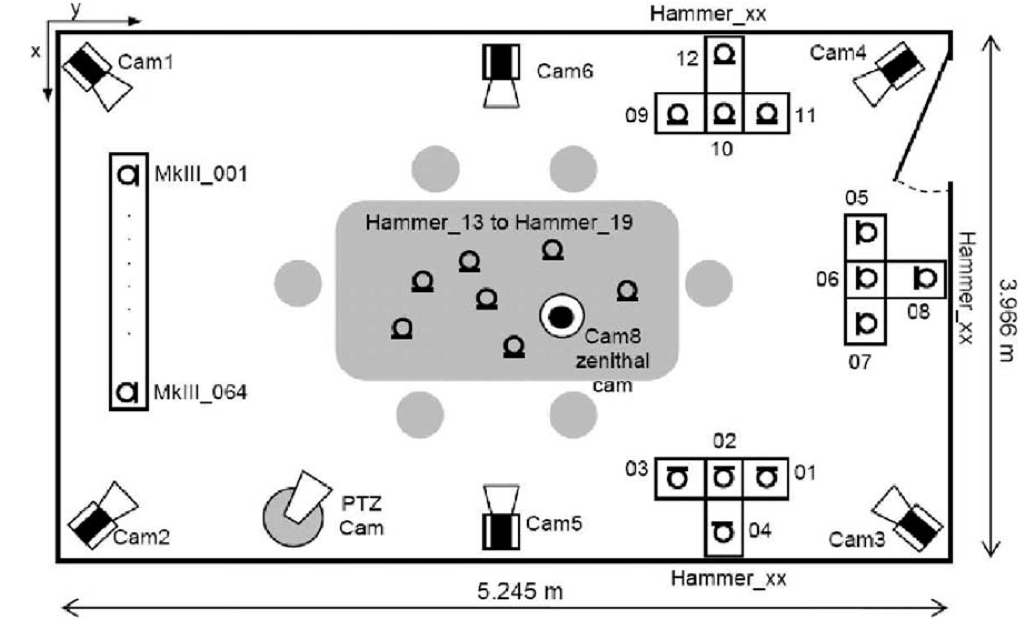
\includegraphics[scale=0.4]{figuras/3.TrabalhosCorrelatos/upc.png}
		\end{center}
		\caption{A configuração do \textit{SmartSpace}~\cite{salah}.}
		\label{upc}
	\end{figure}

Os sensores utilizados e as condições do \textit{SmartSpace} deste projeto são descritos pela Figura \ref{upc}. Os seguintes sensores foram utilizados~\cite{salah}:

	\begin{itemize}
		\item quatro câmeras nos cantos da sala (rotuladas como Cam1 a Cam4 na Figura \ref{upc});
		\item uma camêra \textit{zenithal fish-eye} no telhado (rotulada como Cam8 na Figura \ref{upc});
		\item uma camêra ativa apontadae com zoom para a porta de entrada para capturar as faces das pessoas que entram na sala (rotulada como PTZ na Figura \ref{upc});
		\item um \textit{array} de microfones NIST Mark III de 64 canais ;
		\item três \textit{clusters} de microfone de 4 canais no formato de T;
		\item oito microfones no teto;
	\end{itemize}

O projeto conectar diferentes métodos de rastreamento e reconhecimento prover serviços de recohecimento e rastreamento multimodal no \textit{SmartSpace}. A Figura \ref{workflow} o fluxo de informação no sistema multimodal. O objetivo do sistema é identificar cada usuário ao entrar pela porta e rastrea-lo no ambiente. Para ter um sistema robusto que rastreia e identifica todas as pessoas ao mesmo tempo, utilizaram uma abordagem multimodal~\cite{salah}.

\begin{figure}[hbt]
		\begin{center}
			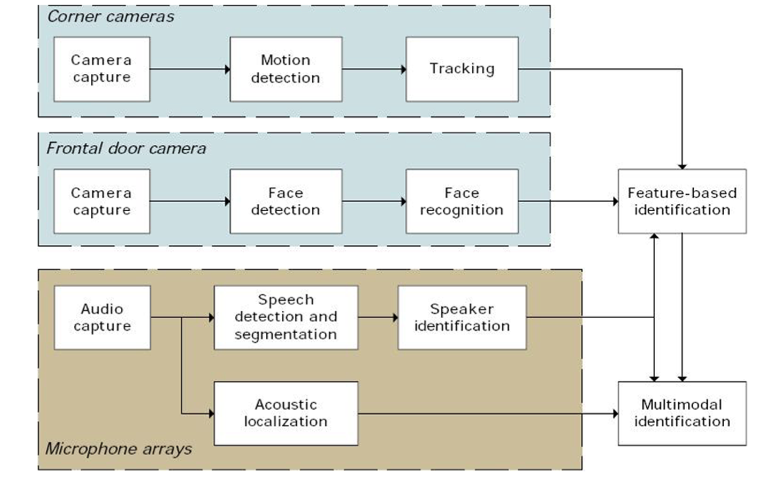
\includegraphics[scale=0.5]{figuras/3.TrabalhosCorrelatos/workflow.png}
		\end{center}
		\caption{\textit{Workflow} da informação na arquitetura do \textit{SmartSpace}~\cite{salah}.}
		\label{workflow}
	\end{figure}

As câmeras no sistema são responsáveis pela detecção de movimento, rastreamento, detecção e reconhecimento facial que são as funcionalidades que nos interessam.

\subsection{Detecção de movimento, Localização e Rastreamento}

A detecção de movimento tenta separar o ``primeiro plano'' do ``fundo''para o seu funcionamento. O método utilizado é baseado na detecção objetos em movimento sob a suposição que imagens em uma cena sem objetos em movimento mostra regularidades, que pode ser modelada utilizando métodos estáticos. O conjunto de treinamento é contruídos por sequências pequenas de gravações \textit{offline} feitas da sala vazia~\cite{salah}.

Para localização e rastreamento foi utilizado a abordagem de um mapa de ocupação probabilística (\textit{probabilistic occupancy map} - POM) simplificado para ambientes internos, onde as trajetórias de movimentos são curtase menos frequentes quando comparadas com trajetórias em ambientes externos~\cite{salah}.

\subsection{Detecção e Reconhecimento Facial}

A detecção de movimento é feita utilizando o método \textit{Viola-Jones} já descrito anteriormente utilizando a biblioteca \textit{OpenCV}. 

Para realizar o reconhecimento facial utiliza uma técnica que aproveita a vantagem que o ambiente é constantemente monitorado e combina a informação de várias imagens para realizar o reconhecimento. As imagens das faces são fornecidas pelo módulo de detecção.
Para cada sequência de imagens, as faces de um mesmo indivíduo são agrupadas. Então, para cada grupo, o sistema compara as imagens com a galeria de imagens~\cite{salah}. 

Uma abordagem baseada em PCA (\textit{Principal Component Analisys}) foi utilizado para comparação entre as imagens.

%%%%%%%%%%%%%%%%%%%%%%%%%%%%%%%%%%%%%%%%%%%%%%%%%%%%%%%%%%%%%%%%%%%%%%%%%%%%%%%%%%%%%%%%%%%%%%%%%%%%%%%%%%%%%%%%%%%%%%%%%%%%%%%%%%%%%%%%%%%%%%%%%%%%%%%%%%%%%%%%%%%%%%%%%%%%%%%%%%%%%%%%%%%%%%%%%%%%%%%%%%%%%%%%%%%%%%%%%%%%%%%%%%%%%%%%%%%%%%%%%%%%%%%%%%%%%%%%%%%%%%%%%%%%%%

\section{Captura de contexto dinâmico e \textit{Arrays} de vídeos distribuídos para \textit{SmartSpaces}}

Esse trabalho apresenta detalhes de um projeto de pesquisa de longo prazo, onde \textit{SmartSpaces} de uma gama de funcionalidades úteis são projetados, construídos e avaliados sistematicamente. Algumas das funcionalidades chave incluem: detecção de intrusos; rastreamento várias pessoas; pose do corpo e análise de postura; identificação de pessoas; modelagem do corpo humano; e análise do movimento~\cite{trivedi}.

O sistema proposto monitora o ambiente em baixa resolução de forma contínua, detectando somente a presença e localização das pessoas e suas dimensões. Formas de acquisição de imagens mais detalhadas são ativadas quando um evento ou atividade de potencial interesse é detectado. Esses eventos serão os focos de atenção do sistema~\cite{trivedi}.

O monitoramente de baixa resolução e de grande área do ambiente é alcançado graças a algumas câmeras de amplo ângulo de visão e estáticas. Com um pequeno número de câmeras PTZ (\textit{pan/tilt/zoom}) ativas, múltiplos focos de atenção podem ser mantidos de forma simultânea~\cite{trivedi}.

Foi desenvolvido uma arquitetura de sistema para o \textit{SmartSpace} chamada DIVA. Ela pode ser vista como uma rede inteligente e ativa de câmeras, onde várias câmeras ão controladas para prover uma ampla gama de funcionalidades~\cite{trivedi}.

	\begin{figure}[hbt]
		\begin{center}
			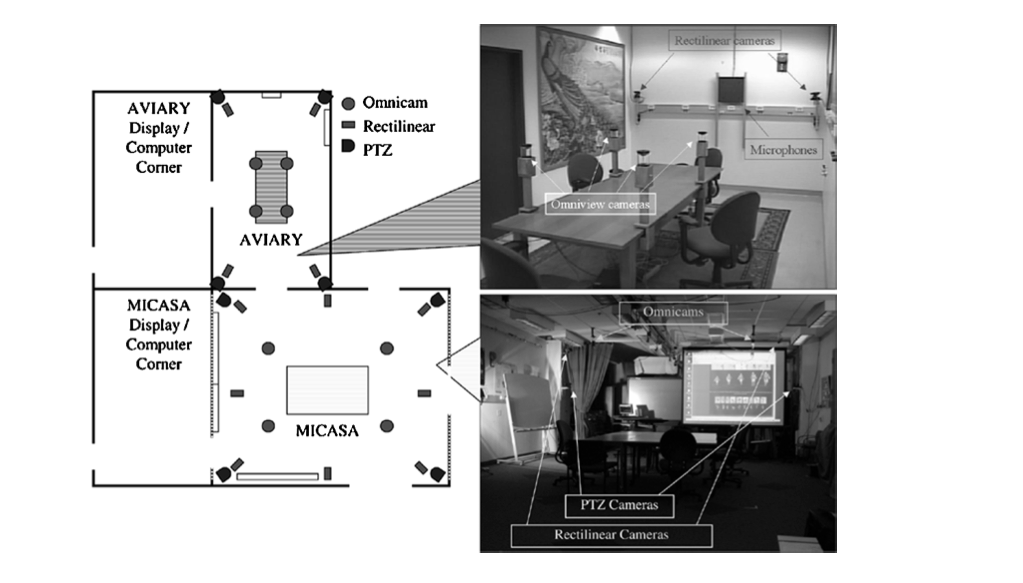
\includegraphics[scale=0.5]{figuras/3.TrabalhosCorrelatos/micasa_aviary.png}
		\end{center}
		\caption{Representação dos \textit{SmartSpaces} MICASA e AVIARY~\cite{trivedi}.}
		\label{micasa_aviary}
	\end{figure}

O projeto inclui dois \textit{SmartSpaces} separados, mas conectados. O primeiro é chamado de AVIARY foi projetado para ser uma pequena sala de conferências. O segundo chamado de MICASA foi projetado para ser uma pequena sala de aula. A Figura \ref{micasa_aviary} mostra fotos dos dois \textit{SmartSpaces} e como estão conectados, além da disposição dos sensores utilizados.

Os sensores na sala AVIARY incluem~\cite{trivedi}:

	\begin{itemize}
		\item uma rede de quatro câmeras omnidirecionais;
		\item quatro câmeras PTZ;
		\item quatro câmeras retilíneas státicas;
		\item dois \textit{arrays} de microfones com quatro microfones cada;
	\end{itemize}

As quatro câmeras ominidirecionais (ODVSs) estão perto dos cantos de uma mesa de reunião, cobrindo o quarto inteiro de dentro para fora, como mostrado na Figura \ref{micasa_aviary}. As câmeras PTZ e retilíneas estão nos ``vértices'' da sala a $\displaysytle 1.4m$ acima do chão. Os dois \textit{arrays} de microfones foram instalados na parede e no teto~\cite{trivedi}.

Um computador é alocado para rastreamento, utilizando imagens das quatro câmeras ominidirecionais ou imagens das quatro câmeras retílinas estáticas. Outro computador é utilizado para analizar os eventos de áudio e de vídeo. Um terceiro computador é utilizado para arquivar \textit{streams} de áudio e vídeo para posterior recuperação~\cite{trivedi}.

O \textit{SmartSpace} MICASA é duas vezes maior que o AVIARY. Os sensores utilizados nessa sala são~\cite{trivedi}:
	
	\begin{itemize}
		\item uma rede de quatro câmeras omnidirecionais;
		\item quatro câmeras PTZ;
		\item oito câmeras retilíneas státicas;
	\end{itemize}

As câmeras omnidirecionais são instaladas no teto, como mostrado na Figura \ref{micasa_aviary}. As câmeras PTZ e quatro câmeras retilíneas foram instaldas de maneira similar ao \textit{SmartSpace} AVIARY. As quatro câmeras retilíneas restantes foram instaladas nas paredes como mostrado como mostrado na Figura \ref{micasa_aviary}. As câmeras nos vértices possuem maior campo de visão para cobrir toda a sala e fazem parte do array de câmeras para rastreamento~\cite{trivedi}.

\subsection{Rastreamento, Detecção de faces e Reconhecimento facial}
 
Foi desenvolvido um sistema em tempo-real que utiliza a rede de camêras omnidirecionais que é responsável pelo rastreamento, detecção das faces e reconhecimento facial. 

O rastreamento baseado na câmeras omnidirecionais é feito detectando a silhuetas das pessoas por meio da subtração do fundo com remoção de sombras.

O vídeo capturado é processado para detecção e reconhecimento de faces como mostrado na Figura \ref{facerec}. Para detecção de faces utiliza o método de segmentação de tom de pele. As imagens resultantes são classificadas para rejeitar as imagens sem faces. Então, o método \textit{Eigenface} é utilizada tanto para classificação da face quanto para reconhecimento. 

	\begin{figure}[hbt]
		\begin{center}
			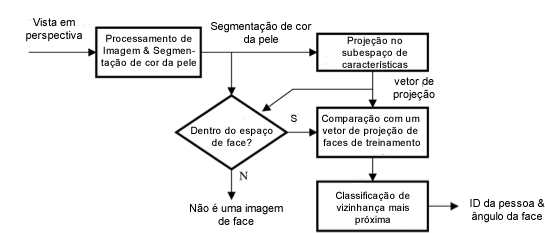
\includegraphics[scale=0.8]{figuras/3.TrabalhosCorrelatos/facerec.png}
		\end{center}
		\caption{Método de detecção e reconhecimento facial~\cite{trivedi}.}
		\label{facerec}
	\end{figure}














































